\begin{frame}
  \frametitle{Généralités}
  \begin{block}{Organisation du semestre}
 \begin{itemize}
   \item CM + TD le Vendredi de 13h00 à 17h00 (C. Koudoro-Parfait \& LG Moreno Jimenez)
   \item Contrôle continu + projet + contrôle terminal
  
  \end{itemize}
  \end{block}
\begin{block}{Ressources}
  \begin{itemize}
  \item \href{http://paris-sorbonne.hosted.exlibrisgroup.com/F?func=find-c&ccl_term=idn=ppn199563403&local_base=MAH01}{TAL et Linguistique Informatique 1}, ISTE Ed. (Mohamed Z. Kurdi) 
  \item Speech and Language Processing (Dan Jurafsky), \url{https://web.stanford.edu/~jurafsky/slp3/} 
  \item Helpdesk : mail ou bureau 206/211 à Serpente (sur RDV)
  \end{itemize}
   \end{block}
\end{frame}

\begin{frame}
  \frametitle{Plan du cours}
\tableofcontents

\end{frame}
\section{Convertir un jupyter notebook en script .py}


\begin{frame}
 \frametitle{Étapes importantes}
\begin{itemize}

\item Commenter le code non essentiel 

\item Refactoriser le code Jupyter Notebook en fonctions

\item Créer des scripts Python pour des tâches associées

\end{itemize} 
\end{frame}

\begin{frame}
 \frametitle{Étapes importantes}
\begin{itemize}
\item Commenter le code non essentiel : \# \\
\ding{220} les parties de programme qui ne \textbf{fonctionnent pas} ou \textbf{expérimentatoires}.

\pause

\item Refactoriser le code Jupyter Notebook en fonctions. Observer votre notebook, n'y a t il pas :\\
\ding{220} des parties de code que vous répétez ?\\
\ding{220} des fonctions que vous répétez inutilement.

\pause

\item Créer des scripts Python pour des tâches associées.\\
\ding{220} Vous pouvez écrire un scripte initiale dans lequel vous appelez un autre script qui va contenir les fonctions que vous souhaitez utiliser
\end{itemize} 
\end{frame}


\begin{frame}
  \frametitle{Enregistrer le fichier au format python - .py}
  Dans la barre de tâche en haut de l'écran jupyter notebook :
  
  
  Aller dans Fichier \ding{219}  Télécharger au format \ding{219}  Python (.py)
  
  \begin{figure}
  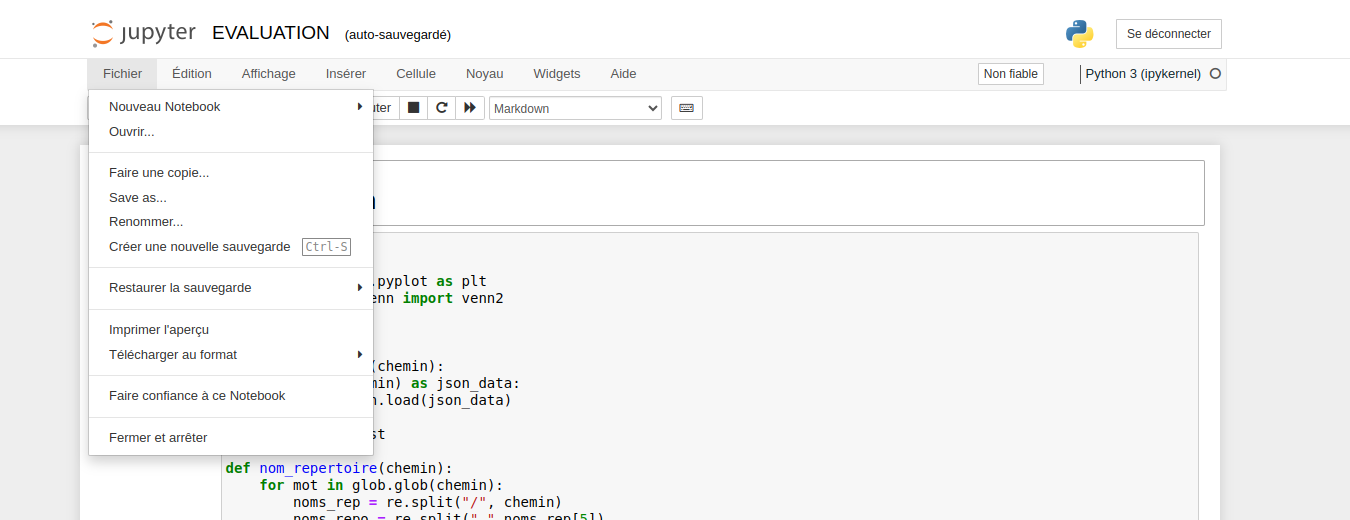
\includegraphics[width=10cm]{images/ynpb_convert_py.png}
  \end{figure}
 
\end{frame}



\begin{frame}
%  \frametitle{}
  
\end{frame}

\section{Spyder un autre environnement }
\begin{frame}  \frametitle{L'explorateur de variable}
  
\end{frame}
\begin{frame}  \frametitle{La console}
  
\end{frame}
\begin{frame} \frametitle{L'Éditeur}
  
\end{frame}
\begin{frame}
  \frametitle{}
  
\end{frame}
\begin{frame}
%  \frametitle{}
  
\end{frame}

\section{Listes, set et match !}
\begin{frame}
%  \frametitle{}
  
\end{frame}
\begin{frame}
%  \frametitle{}
  
\end{frame}
\begin{frame}
%  \frametitle{}
  
\end{frame}
\begin{frame}
%  \frametitle{}
  
\end{frame}\begin{frame}
%  \frametitle{}
  
\end{frame}






